\subsection{Space Shift Keying Modulation}
Space Shift Keying (SSK) Modulation \cite{5165332} is a technique where \textit{antenna indices are used as the only means to relay information}. Given $K$ the number of antenna of the actors in the system, we can send $log_2(K)$ bits by mapping each combination of bits to a specific antenna.
\footnote{This may seem rather unoptimized, as we use only one antenna instead of combinations of them. To see a more general approach, the authors also wrote the paper \cite{4699782}, where they discuss a more general approach.}

\begin{figure}[H]
  \centering
  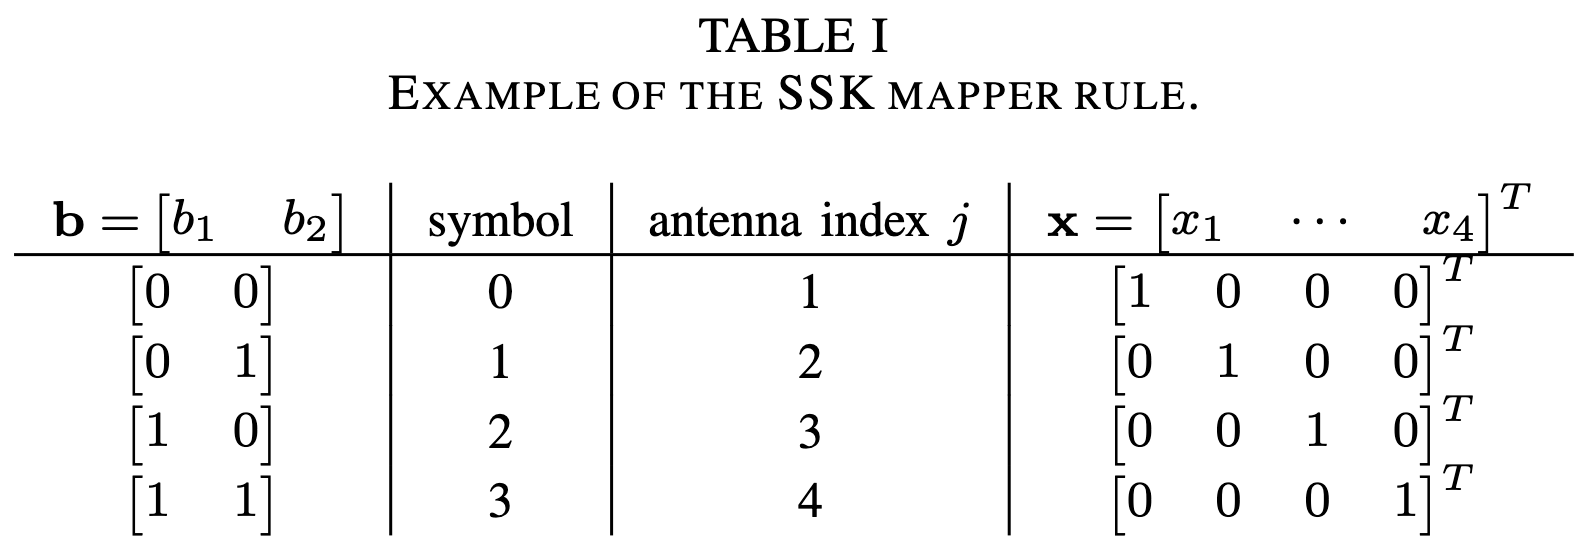
\includegraphics[width=\linewidth]{imgs/ssk_conversion_table.png}
  \caption{SSK conversion table}
  \label{fig:ssk_conversion_table}
\end{figure}

\subsubsection{Direct Detection}
Given a channel gain matrix $B \in \C^{NxN}$ and the input vector $x$ with only one element equal to $1$, the signal received is $y = Bx + \sigma^2$. To understand the antenna index which sent the message, we need to find the column $b_j$ which is most similar to $y$.

\begin{equation}
  j = arg\ max_j\ p_y (y | x_j, B) = arg\ min_j\ || y - b_j ||^2
\end{equation}

\subsubsection{Diagonalized Reflection Detection}
Following \cite{9328149}, for a reflected signal we have $y = GPHx + \sigma^2$. Given that $GPH$ is a diagonal matrix and $x$ has only one element equal to $1$, the resulting vector $GPHx$ will still be a vector with only one element non zero. Adding noise, to find the antenna index we search for the biggest value in the vector.

\begin{equation}
  j = arg\ max_j\ y_j
\end{equation}